\chapter{Prehľad problematiky}
\label{kap:kapitola1}
Prehľad definícií sme čerpali z \cite{Bru92}, \cite{Bru81}, \cite{doCarmo17} a \cite{Ode20}.

\section{Jednoparametrický systém}
Ak nakreslíme kružnice so stredom na x-ovej osi s polomerom 1, ako na obr. \ref{fig:system}, pohľad nám upútajú úsečky $y = \pm 1$ pre $ x \in [-2,2]$ idúce ponad a popod systém kružníc.

\begin{figure}[h]
	\centering
	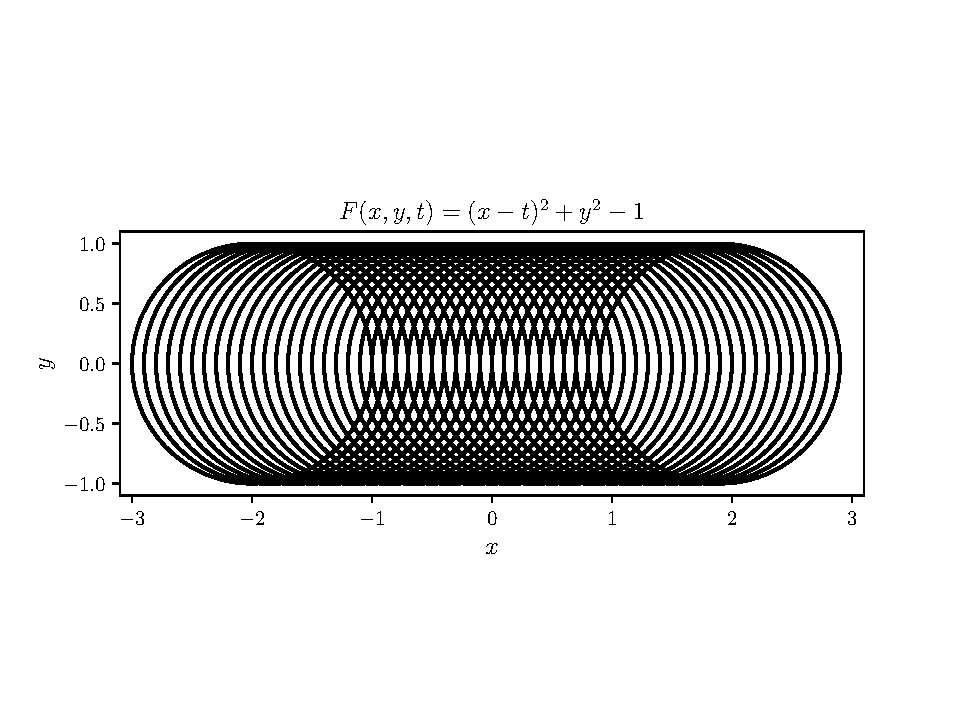
\includegraphics[trim={0.5cm 2.8cm 0.5cm 3.3cm},clip]{images/system.pdf}
	\caption[Systém kružníc.]{Systém kružníc.}
	\label{fig:system}
\end{figure}

Každá z týchto úsečiek sa dotýka každej kružnice v jednom bode a v tomto bode majú spoločnú dotyčnicu. V nasledovnom texte túto myšlienku matematicky opíšeme, na základe nej zostrojíme tzv. obálku systému kriviek alebo plôch a porovnáme prístupy ich výpočtu. Budeme pracovať v reálnom vektorovom priestore so štandardným skalárnym súčinom, teda v euklidovskom priestore $\mathbb{E}^{n}$, rozmeru $n = 2, 3.$ Najprv ilustrujeme príklady obálok a ich výpočet pre $ n = 2,$ neskôr pre $n = 3.$ Po celý čas predpokladáme, že všetky zobrazenia sú dostatočne veľakrát diferencovateľné a pre prehľadnosť zápisov vynechávame parametre, ak sú z kontextu zrejmé.

%Vo všeobecnosti, začneme v $\mathbb{E}^2$ s jednoparametrickým systémom kriviek daným funkciou, v $\mathbb{E}^3$ máme jednoparametrický systém plôch.

\begin{definition}
Nech $F \colon \mathbb{R}^{n} \times I \rightarrow \mathbb{R}$ je funkcia v premenných $ x_{1}, x_{2}, \ldots, x_{n} $ a v parametri $t$, kde $I \subseteq \mathbb{R}$ je interval. Definujeme jednoparametrický systém nadplôch ako systém množín 
$$
\mathcal{F} = \{ (x_{1}, x_{2}, \ldots, x_{n}) \in \mathbb{R}^{n} \mid  \ F(x_{1}, x_{2}, \ldots, x_{n}, t) = 0, \ t \in I \}.
$$
\end{definition}

V $n = 2$ budeme pre lepšiu prehľadnosť značiť premenné $x_{1}, x_{2}$ ako $x, y,$ pre $n = 3$ pribudne $x_{3}$ ako $z.$ Pre lepšiu prehľadnosť neskôr označíme dvojicu $(x,y)$ alebo trojicu $(x,y,z)$ ako $X$, potom
$\mathcal{F} = \{ X \in \mathbb{R}^{n} \mid \ F(X, t) = 0, \ t \in I \}. $

Pre horeuvedený prípad, vizualizovaný na obr. \ref{fig:system}, teda máme jednoparameterický systém kružníc so stredmi kružníc, ktoré ležia na úsečke parametrizovanej $(t,0)$ pre $t \in [-2,2]$ a konštantným polomerom pre každú kružnicu $r = 1$ daný implicitnou funkciou
$$ \mathcal{F} = \{ (x, y) \in \mathbb{R}^{2} \mid \ F(x, y, t) = 0, \ t \in [-1,1] \}, $$
kde
$$ F(x, y, t) = (x - t)^2 + y^2 - 1.$$

Systém budeme ilustrovať zobrazením niektorých prvkov systému pre diskrétne hodnoty parametra $t$. Pre $t = -2$ je zodpovedajúci prvok systému $\mathcal{F}_{-2} \in \mathcal{F}$  kružnica s implicitnou rovnicou
$$ F_{-2}(x, y) = F(x, y, -2) = (x + 2)^2 + y^2 - 1. $$
Často budeme pre pevný parameter $t_0$ označovať prislúchajúcu rovnicu $F_{t_0}(X)$ a množinu bodov, ktoré rovnicu spĺňajú označíme $\mathcal{F}_{t_0}.$

\begin{figure}[h]
	\centering
	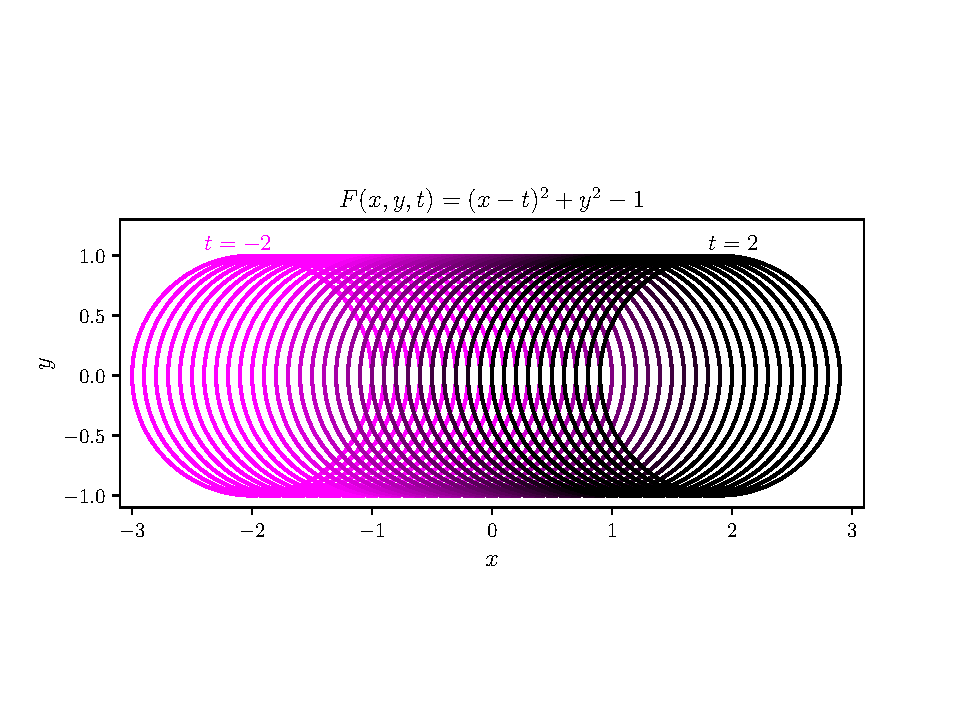
\includegraphics[trim={0.5cm 2.5cm 0.5cm 3cm},clip]{images/elements.pdf}
	\caption[Zobrazenie prvkov systému.]{Systém je zobrazený na intervale $[-2,2]$ s krokom  $\Delta t = 0,1$. Ružovou farbou je vyznačená kružnica systému v parametri $t=-2$, čiernou farbou v parametri $t = 2$, v hodnotách parametrov medzi nimi je farba kružnice lineárne interpolovaná. }
	\label{fig:one_element_of_system}
\end{figure}

\section{Obálka jednoparametrického systému nadplôch}
Najskôr definujeme obálku jednoparametrického systému kriviek v $\mathbb{E}^2$. Uvedieme charakterizáciu obálok, ktorú možno použiť na výpočet pre jednoduchšie jednoparametrické systémy. Následne túto charakterizáciu použijeme ako definíciu pre obálku jednoparametrického systému plôch v $\mathbb{E}^n$.

\begin{definition}
Definujme gradient funkcie $F \colon \mathbb{R}^2 \times I \rightarrow \mathbb{R}$ vzhľadom na $x$ a $y$ ako
$$\nabla F(x, y, t) = \left(\frac{\partial F}{\partial x}(x, y, t), \frac{\partial F}{\partial y}(x, y, t) \right).$$ 
\end{definition}

\begin{definition}
\label{definicia}
Obálkou systému kriviek $ \mathcal{F} $ je parametrizovaná krivka $\gamma(t) \colon J \subseteq I \rightarrow \mathbb{R}^{2}$ taká, že 
\begin{enumerate}
\item $\gamma(t) \in \mathcal{F}_{t} \text{ pre všetky } t \in J,$
\item $\dot{\gamma}(t) \perp \nabla F \left( \gamma(t), t \right).$
\end{enumerate}
\end{definition}

Obálka $\gamma(t)$ sa dotýka každej krivky zo systému $F(x,y,t)$ v bode $(x, y)$  pre nejaké $t$ a v tomto bode má s krivkou zo systému rovnakú dotyčnicu. To znamená, že každý bod obálky ${\gamma}(t) = (\gamma_{1}(t),\gamma_{2}(t))$ spĺňa rovnicu systému $F(\gamma_{1}(t),\gamma_{2}(t),t)=0$ pre nejaké $t,$ a~teda platí prvá podmienka $\gamma(t) \in \mathcal{F}_{t}$. Gradient funkcie $ \nabla F(x,y,t)$ možno geometricky interpretovať ako normálový vektor k $F(x,y,t)$ v regulárnom bode $(x,y)$ a parametri $t$. V spoločnom bode $(x,y)$ a parametri $t$ požadujeme lineárnu závislosť dotykového vektora obálky $\gamma(t)$ a systému $F(x,y,t), $ z čoho dostávame $\dot{\gamma}(t) \perp \nabla F \left( \gamma(t), t \right), $ druhú podmienku v definícii obálky. Interval $J,$ na ktorom dostávame výslednú obálku môže byť menší ako interval $I,$ na ktorom bol definovaný systém kriviek, teda máme $J \subseteq I.$

Pre všetky $(x, y, t)$ predpokladáme, že  $\nabla F(x,y,t) \neq \vec{0}. $  Ak by bol gradient $\nabla F(x,y,t) $ v nejakom bode nulový, nevieme jednoznačne nájsť dotykový vektor systému $F(x, y, t).$ 

\begin{theorem}
Regulárna krivka $\gamma(t) \colon J \subseteq I \rightarrow \mathbb{R}^{2}$ kde $t \in J  \subseteq I$ je obálkou jednoparametrického systému $\mathcal{F}$ práve vtedy, keď spĺňa:
\begin{enumerate}
\item $F(\gamma(t), t) = 0, $ 
\item $\dfrac{\partial F}{\partial t}(\gamma(t), t) = 0.$
\end{enumerate}
\end{theorem}

\begin{proof}
Táto odlišná charakterizácia je ekvivalentná definícii, ktorú sme postavili na geometrických podmienkach. Stačí zistiť korešpondenciu podmienok.
\begin{enumerate}
\item Ako sme už vysvetlili, každý bod obálky ${\gamma}(t) = (\gamma_{1}(t),\gamma_{2}(t))$ spĺňa rovnicu jednoparametrického systému $F(\gamma_{1}(t),\gamma_{2}(t),t)=0$ pre nejaké $t,$ teda podmienky 
$$ F(\gamma(t), t) = F(\gamma_{1}(t), \gamma_{2}(t), t) = 0$$
a
$$\gamma(t) \in \mathcal{F}_{t}$$
sú ekvivalentné.
\item Derivujme $F(\gamma_{1}(t),\gamma_{2}(t), t)$ podľa parametra $t,$ kde $ \dot{\gamma}(t) = ( \dot{\gamma_{1}}(t), \dot{\gamma_{2}}(t) ).$
$$ \frac{\partial F}{\partial x}(\gamma_{1}(t),\gamma_{2}(t),t) \cdot \dot{\gamma_{1}}(t)+\frac{\partial F}{\partial y}(\gamma_{1}(t),\gamma_{2}(t),t) \cdot \dot{\gamma_{2}}(t)+\frac{\partial F}{\partial t}(\gamma_{1}(t),\gamma_{2}(t),t) \cdot 1 = 0. $$
Nakoľko požadujeme, aby gradient funkcie $\nabla F(\gamma_{1}(t),\gamma_{2}(t),t)$ bol kolmý na $\dot{\gamma}(t) \text{ tak}$
$$ \langle \nabla F(\gamma_{1}(t),\gamma_{2}(t),t), \dot{\gamma}(t) \rangle = 0,$$
a teda platí
$$ \frac{\partial F}{\partial x}(\gamma_{1}(t),\gamma_{2}(t),t) \cdot \dot{\gamma_{1}}(t)+\frac{\partial F}{\partial y}(\gamma_{1}(t),\gamma_{2}(t),t) \cdot \dot{\gamma_{2}}(t) = 0, $$
z čoho dostávame
$$ \frac{\partial F}{\partial t}(\gamma_{1}(t),\gamma_{2}(t),t) = 0. $$ 
\end{enumerate}
\end{proof}

%Obálka sa počíta riešením rovníc
%\begin{align*}
%F(x, y, t) &= 0, \\
%\frac{\partial F}{\partial t}(x,y,t) &= 0. \\
%\end{align*}

Často sa v literatúre môžeme stretnúť s rôznymi opismi obálky, ktoré však bez ďalších predpokladov nemusia definovať rovnakú množinu bodov. Príkladom je ďalšia charakterizácia obálky ako množiny limitných bodov prienikov kriviek systému. Vzťahy medzi jednotlivými charakterizáciami možno nájsť v \cite{Bru81}.  

Dokonca, daný systém nemusí mať obálku. Príkladom sú sústredné kružnice s rastúcim polomerom.

\begin{example} 
Obálku systému sústredných kružníc pre $t \in I=[\frac{1}{100},2]$ rátame ako riešenie systému rovníc
\begin{align*}
F(x, y, t) &= x^2 + y^2 - t, \\
\frac{\partial F}{\partial t}(x,y,t) &= -1. \\
\end{align*}
Z druhej rovnice máme $t=-1 \neq 0,$ teda systém nemá riešenie. Aj keď by sa nám mohlo zdať, že by obálkou mohli byť body kružnice s najväčším polomerom $\mathcal{F}_2$ a kružnice s najmenším polomerom $\mathcal{F}_{\frac{1}{100}}$, práve podmienka existencie takej krivky $\gamma(t),$ ktorá by patrila do systému kružníc $\mathcal{F}$ pre všetky $t$ z intervalu $J \subseteq  I, $ nie je splnená.
\end{example}

\begin{figure}[h]
	\centering
	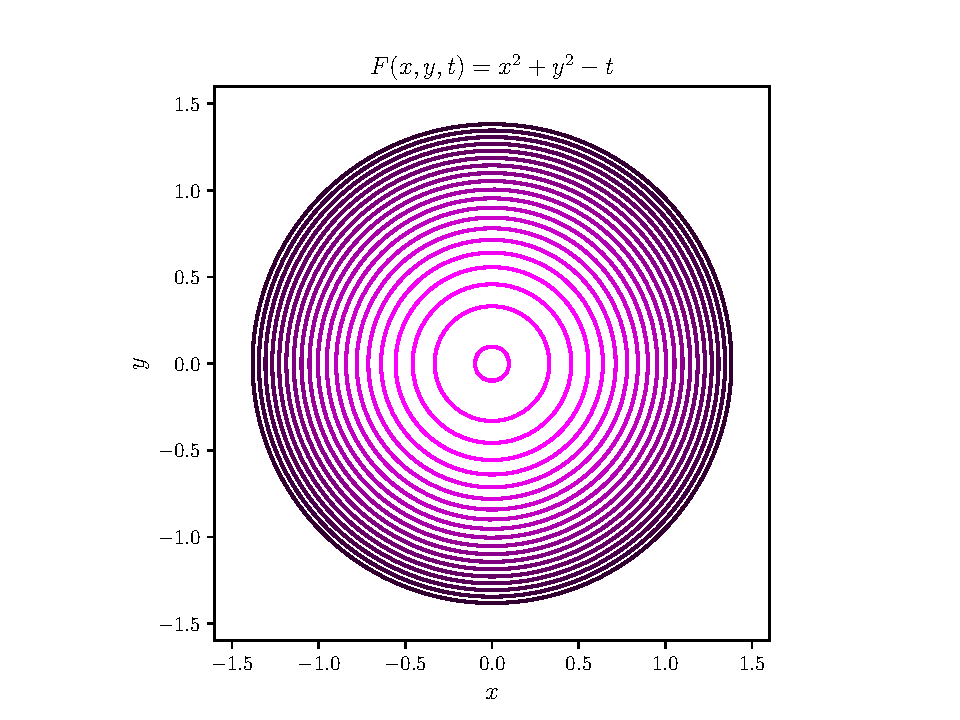
\includegraphics[trim={0 0.35cm 0 0.85cm},clip, width=0.9\textwidth]{images/concentric_circles.pdf}
	\caption[Sústredné kružnice.]{Sústredné kružnice na intervale $[\frac{1}{100},2]$ a krokom $\Delta t = 0,1$.}
	\label{fig:concentric_circles}
\end{figure}

Prístup, ktorý sme využili pre jednoparametrický systém kriviek, možno zovšeobecniť pre ľubovoľný jednoparametrický systém plôch v $\mathbb{E}^n.$

\begin{definition}{\textbf{\textup{(Charakterizácia.)}}}
\label{charakterizacia}
Obálkou jednoparametrického systému plôch $ \mathcal{F} $ je množina bodov $\mathcal{E}$ daná
$$\mathcal{E} = \{ X \in \mathbb{R}^{n} \colon \exists t \in \mathbb{R} \mid F(X, t) = \frac{\partial F}{\partial t}(X, t) = 0 \}.$$
\end{definition}

Ak by sme chápali obálku podľa definície ako množinu bodov, problém by sme mohli riešiť ako systém nelineárnych rovníc v parametri $t,$ kde chceme z rovníc 
\begin{align*}
F(x,y,t) &= 0, \\
\frac{\partial F}{\partial t}(x, y, t) &= 0. \\
\end{align*}
eliminovať $t.$ Na riešenie nelineárneho systému dvoch rovníc síce existujú pokročilé nástroje, no eliminovaním parametra $t$ strácame informáciu o tom, na akom intervale $I$ je obálka definovaná. 

\begin{example}
Pre náš príklad $ F(x, y, t) = (x - t)^2 + y^2 - 1 = 0 $ máme 
$$\frac{\partial F}{\partial t}(x, y, t) = 2(t-x) = 0. $$
Ak $t = x, $ tak $y^2 = 1.$ Teda obálka je podľa tejto charakterizácie $ y = \pm 1, $ ako sme očakávali.
\end{example}

\begin{figure}[h]
	\centering
	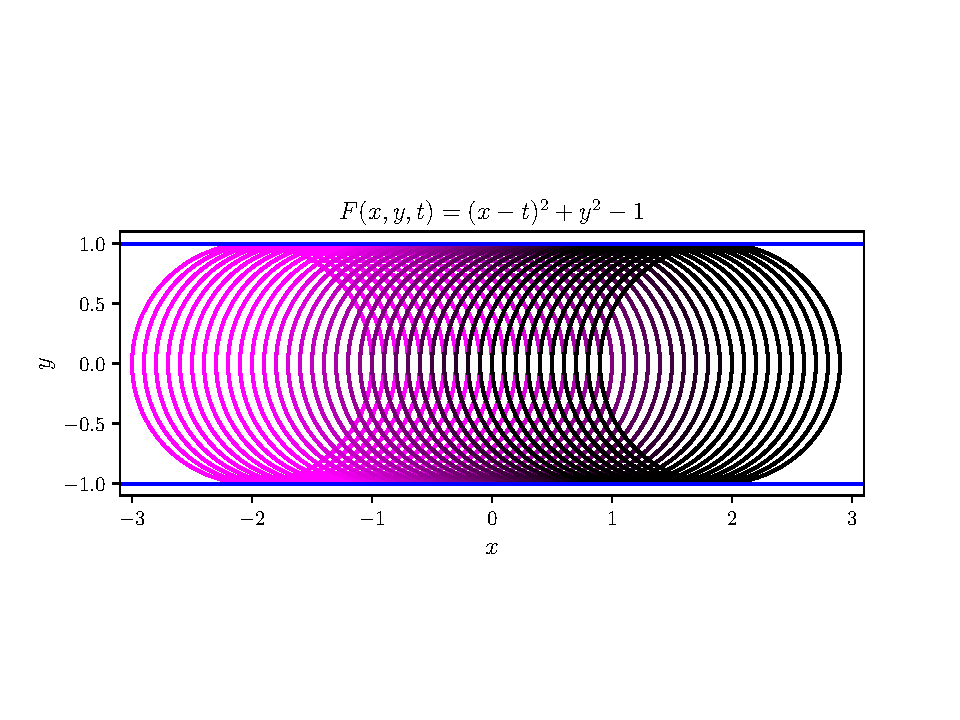
\includegraphics[trim={0.5cm 2.8cm 0.5cm 3.3cm},clip]{images/system_with_envelope_unlimited_domain.pdf}
	\caption[Obálka systému podľa charakterizácie.]{Obálka systému podľa charakterizácie \ref{charakterizacia}.}
	\label{fig:system_with_envelope_unlimited_domain}
\end{figure}

V skutočnosti sú obálkou úsečky $y=\pm 1$ definované na intervale $[-2,2]$. Tento problém možno ošetriť tak, že budeme uvažovať systémy kriviek, ktoré sú v parametri $t$ definované na celej reálnej priamke $\mathbb{R}$. 

\begin{figure}[h]
	\centering
	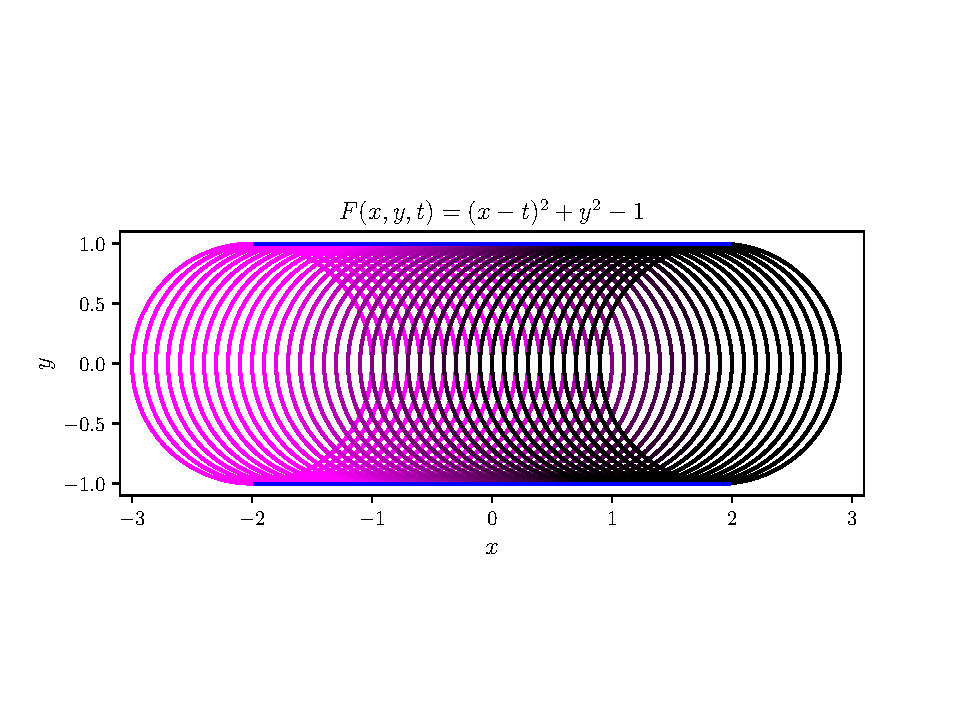
\includegraphics[trim={0.5cm 2.8cm 0.5cm 3.3cm},clip]{images/system_with_correct_envelope.pdf}
	\caption[Obálka systému podľa definície.]{Obálka systému podľa definície \ref{definicia}.}
	\label{fig:system_with_correct_envelope}
\end{figure}

Ďalšou otázkou, ktorá prirodzene vzniká je, či patria aj časti kriviek jednoparametrického systému v koncových bodoch intervalu do obálky. Podľa defínicie a charakterzácie nie. Ak by sme predsa len koncové časti pridali, mohli by sme systém v prípadoch kružníc, elíps, sfér a elipsoidov ohraničiť akousi kontúrou systému. Na obr. \ref{fig:nanuk} sa nachádza vizualizácia systému s jeho kontúrou vytvorenou z obálky systému a polkružnicami v parametroch $t=-2$ a $t=2.$

\begin{figure}[H]
	\centering
	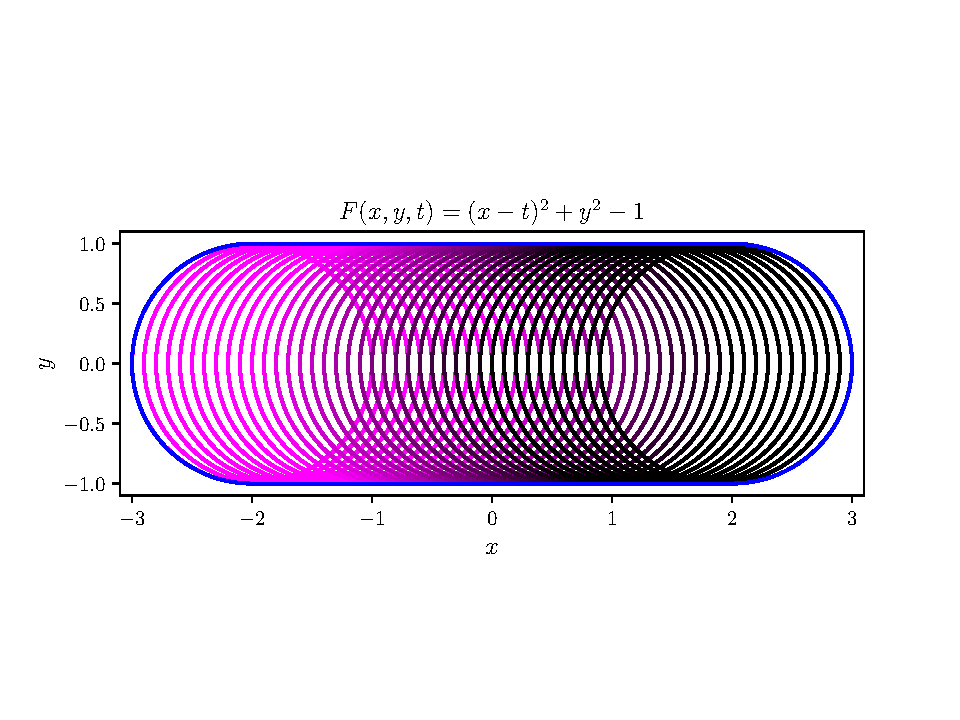
\includegraphics[trim={0.5cm 2.8cm 0.5cm 3.3cm},clip]{images/nanuk.pdf}
	\caption{Kontúra systému.}
	\label{fig:nanuk}
\end{figure}

\begin{example}
\label{example:too_complicated_equations}
Počítajme obálku systému kriviek, znázorneného na obrázku \ref{fig:too_complicated_equations}, ktorý je daný vzťahmi
\begin{align*}
F(x,y, t) &= \dfrac{x^2}{(t^2 + 1)^2} + (y - 2t)^2 - 1, \\
\dfrac{\partial F}{\partial t}(x, y, t) &= -\dfrac{4x^2t}{\left(t^2+1\right)^3}-4\left(y-2t\right). \\
\end{align*}
Vynásobením prvej rovnice $ \lambda(t) = (t^2 + 1)^2$ a derivovaním získavame
\begin{align*}
F^\lambda &= 4 t^6 - 4 t^5 y + t^4 y^2 + 7 t^4 - 8 t^3 y + 2 t^2 y^2 + 2 t^2 - 4 t y + x^2 + y^2 - 1, \\
F_t^\lambda &= 24t^5-20yt^4+4y^2t^3+28t^3-24yt^2+4y^2t+4t-4y. \\
\end{align*}
Na obrázku \ref{fig:too_complicated_equations} je znázornený tento systém elíps pre $t \in [-2,2]$ s krokom $\Delta t=0.1$. Obálku nájdeme ako riešenie rovníc $F^\lambda \cap F_t^\lambda. $ Rovnice sú však príliš vysokého stupňa v parametri $t$, preto nevieme implicitnú rovnicu obálky bez vhodného nástroja vyjadriť. V ďalšej časti rozoberieme známe prístupy výpočtu.
\end{example}

\begin{figure}[h]
	\centering
	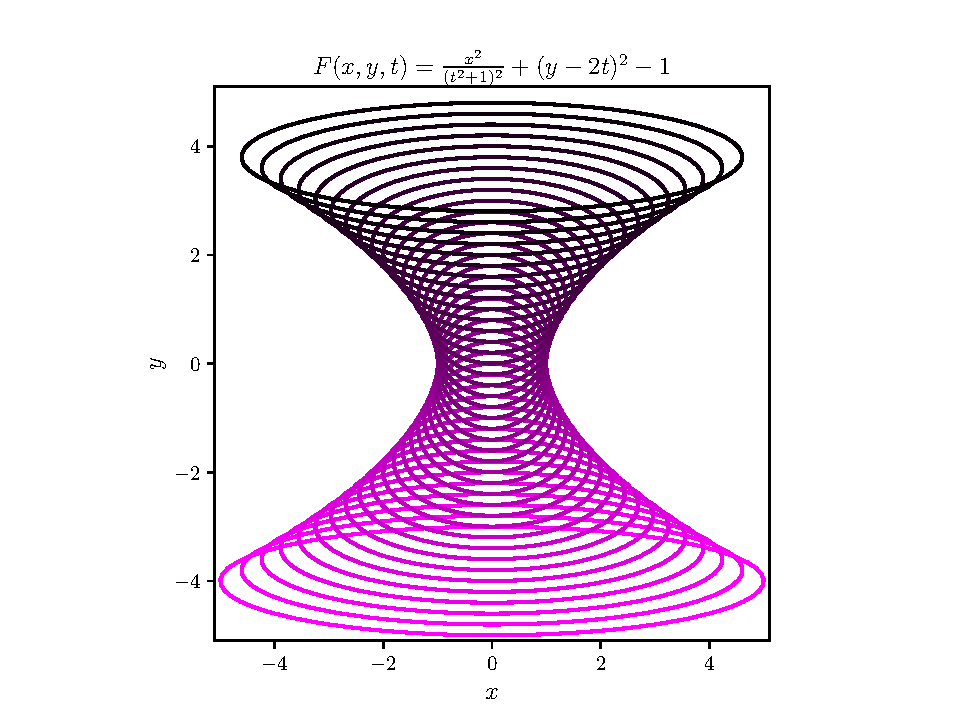
\includegraphics[trim={0 0.35cm 0 0.85cm},clip, width=\textwidth]{images/too_complicated_equations.pdf}
	\caption[Systém elíps.]{Systém elíps, pre $t=-2$ ružová elipsa, pre $t=2$ čierna elipsa.}
	\label{fig:too_complicated_equations}
\end{figure}

\section{Výpočet obálky}
Vo väčšine prípadov sú rovnice charakterizujúce obálku systému plôch príliš vysokého stupňa v parametri $t$ a nedokážeme z nich ľahko odvodiť rovnicu obálky, preto pristupujeme aj k numerickým riešeniam. Spoľahlivá aproximácia obálky je jednou z aktuálnych výskumných tém. Na začiatok si však rozoberme existujúce analytické prístupy. Naledujúce prístupy sú prevzaté z \cite{Vra22}.
\subsection{Prístup algebraickej geometrie}
Dokonca aj v prípade jednoduchého príkladu \ref{example:too_complicated_equations}, obe polynomické rovnice charakterizujúce obálku sú vysokého stupňa v parametri $t$, preto je odstránenie parametera $t$ náročné bez vhodného nástroja. Štandardným aparátom na túto úlohu sú Gröbnerove bázy. Gröbnerove bázy sú kľúčovým pojmom v algebraickej geometrii a počítačovej algebre. Ide o špeciálnu množinu polynómov vo viacerých premenných, ktoré majú niekoľko dôležitých vlastností a zohrávajú kľúčovú úlohu pri riešení rôznych matematických problémoch vrátane riešenia sústav polynomických rovníc, zjednodušovania polynómov a dokazovania rôznych algebraických tvrdení. Vybudovanie tejto teórie je pomerne zdĺhavé, preto odkážeme na bohaté teoretické pozadie v \cite{Chalm}.
%Najprv vypočítame Gröbnerovu bázu Buchbergerovým algoritmom pre ideál generovaný sústavou polynomických rovníc, ktorá obsahuje všetky premenné vrátane tej, ktorú chceme eliminovať. Z Gröbnerovej bázy vyberieme polynómy, ktoré obsahujú premennú, ktorú chceme eliminovať. Tieto polynómy použijeme na vyjadrenie tejto premennej v závislosti od ostatných premenných. Po vyriešení nových rovníc získame výraz, ktorý opisuje vzťah medzi zvyšnými premennými a eliminovanou premennou. Týmto spôsobom úspešne eliminujeme premennú.
%Pokúsme sa vypočítať Gröbnerovu bázu príkladu \ref{example:too_complicated_equations} vzhľadom na lexikografické usporiadanie monómov $t > x > y $. 
Keďže výpočet Gröbnerovej bázy trvá pomerne dlho, neuvádzame postup a výsledok možno nájsť v  \altref{kap:priloha1}{Prílohe A}. 

%Gröbnerova báza vzhľadom na iné usporiadanie, napr. grevlex je zvyčajne vypočítaná oveľa rýchlejšie a jej polynómy majú krajšie koeficienty, no na druhej strane, tento prístup nie je vo všeobecnosti možné použiť na odstránenie premennej $t$ z rovníc. 
%Spôsob, ako nájsť polynóm, ktorý leží v prvom eliminačnom ideáli, ktorý je nezávislý na Gröbnerovej bázach a monómických usporiadaniach, využíva teóriu rezultantov. 

Gröbnerovu bázu je možné určiť vzhľadom na usporiadanie monómov, existujú aj iné metódy na riešenie polynomických rovníc, ktoré nie sú závislé na usporiadaní monómov. Jednou z metód je výpočet rezultantu, determinant špeciálnej matice polynómov.
Hoci výpočet determinantov veľkých matíc je výpočtovo aj časovo náročný problém, poznáme metódy, ako vypočítať determinant efektívnejšie. 
Navyše táto metóda, rovnako ako metóda založená na eliminačnej teórii s použitím Gröbnerových báz, nám vypočíta správnu obálku len vtedy, ak uvažujeme parameter $t$ jednoparametrického systému z celej reálnej priamky. 

%Ak obmedzíme oblasť parametra na interval, tak obálka zvyčajne nemôže byť daná implicitnou rovnicou, a preto je potrebné nájsť nejakú parametrizáciu obálky. 

Pri použití rezultantov máme lepšiu kontrolu nad zložitosťou výpočtu. Pre dané dva polynómy totiž vieme, ako sa konštruuje rezultant, a tak vieme odhadnúť, s akými veľkými polynómami sa bude počas výpočtu manipulovať, avšak pri hľadaní Gröbnerovej bázy je ťažké odhadnúť, aké zložité polynómy sa behom algoritmu vyskytnú.

V príklade \ref{example:too_complicated_equations} uvedieme výsledný polynóm $Res(F^\lambda , F_t^\lambda , t)$ a na obr. \ref{fig:resultant} obálku nájdenú pomocou rezultantu. 

$ Res(F^\lambda , F_t^\lambda , t) = 191102976x^{10} + 262144x^8y^6 - 9584640x^8y^4 + 83165184x^8y^2 - 633470976x^8 - 16384x^6y^{10} - 81920x^6y^8 - 14483456x^6y^6 - 113311744x^6y^4 + 96419840x^6y^2 + 698368000x^6 - 16384x^4y^{12} - 294912x^4y^{10} - 2998272x^4y^8 - 18284544x^4y^6 - 74956800x^4y^4 - 184320000x^4y^2 - 256000000x^4. $

%[trim={0 0.35cm 0 0.85cm},clip

\begin{figure}[h]
	\centering
	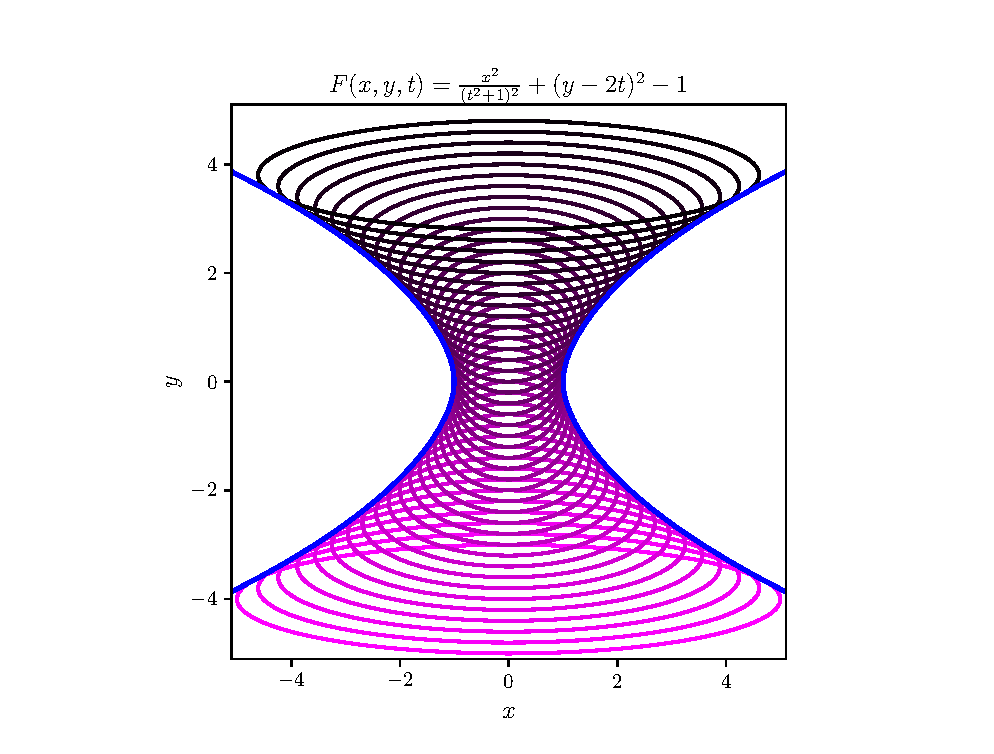
\includegraphics{images/resultant.eps}
	\caption[Obálka nájdená rezultantom.]{Modrou farbou je znázornená obálka vypočítaná rezultantom.}
	\label{fig:resultant}
\end{figure}


\subsection{Prístup projektívnej geometrie}
Body duálneho projektívneho priestoru $\mathbb{P}^3 $ možno stotožniť s nadrovinami v $\mathbb{R}^3$. Plochu v duálnom projektívnom priestore možno teda interpretovať ako množinu všetkých jej dotykových nadrovín. Pomocou duálneho prístupu sa dá dokázať, že obálky jednoparametrických systémov sú pre racionálne vstupné údaje racionálne. Potrebné vybudovanie teórie možno nájsť v \cite{Pott01}, z čoho čerpajú články s mnohými výsledkami \cite{Pet08}, \cite{Pet98} a príklady pre výpočet obálky možno nájsť v \cite{Vra22}.
\begin{example}
Uvažujme dva systémy kružníc $\mathcal{F}$ s konštantným polomerom $\frac{1}{2}$ a $\mathcal{G}$ s funkciou polomeru $\frac{t}{2}$, ktorých stredy ležia na rovinnej krivke $m(t) = (t^3, t^2)$, kde $t \in \mathbb{R}.$
So systémom
$$ \mathcal{F} = \{ X \in \mathbb{R}^2 \mid (x - t^3)^2 + (y - t^2)^2 - \frac{1}{4} = 0, t \in \mathbb{R} \}.$$
korešponduje krivka $m_1 = (t^3, t^2, \frac{1}{2})\subset \mathbb{R}^3$.
Pre
$$ \mathcal{G} = \{ X \in \mathbb{R}^2 \mid (x - t^3)^2 + (y - t^2)^2 - \frac{t^2}{4} = 0, t \in \mathbb{R} \}$$
máme krivku $m_2(t) = (t^3, t^2, \frac{t}{2}).$
Kružnice zodpovedajúce $t < 0$ sú negatívne orientované, pre $t > 0$ pozitívne orientované, pre $t = 0$ je prvok $\mathcal{F}_0 \in \mathcal{F}$ bod $ (0, 0) \in m(t), $ čo je kružnica s nulovým polomerom a bez určenej orientácie.
Krivka $m(t)$ je ortogonálna projekcia oboch kriviek $m_1$ a $m_2$ a často sa nazýva stredná os \textit{(medial axis)} jednoparametrického systému.
\end{example}

Rovnakým spôsobom môžeme definovať jednoparametrický systém sfér v $\mathbb{R}^3$ ako obraz kriviek v $\mathbb{R}^4$.
Jedným z dôležitých výsledkov je, že pomocou tohto prístupu možno rozhodnúť o reálnosti obálky a to tak, že systém korešpondujúci s krivkou $m(t) \subset \mathbb{R}^{n+1}$ má reálnu obálku práve vtedy, keď pre všetky $t \in I $ platí 
$$\langle \dot{m}(t), \dot{m}(t) \rangle \geq 0$$ 
a rovnosť platí len pre izolované hodnoty $t$, kde za skalárny súčin vezmeme pseudo-skalárny súčin vyjadrený ako $\langle \dot{m}(t), \dot{m}(t) \rangle = m_1^2(t) + m_2^2(t) + \ldots + m_n^2(t) - m_{n+1}^2(t).$

Pre príklad tak 4 máme
\begin{align*}
&\langle \dot{m}_1(t), \dot{m}_1(t) \rangle = 9t^4 + 4t^2 \geq 0, \text{ pre } t \in \mathbb{R}, \\
&\langle \dot{m}_2(t), \dot{m}_2(t) \rangle = 9t^4 + 4t^2 - \frac{1}{4} \geq 0, \text{ pre } t \in \mathbb{R} \setminus \{ (-0.236, 0) \cup( 0, 0.236) \},
\end{align*}
preto na týchto intervaloch existuje reálna obálka systémov $\mathcal{F}$ a $\mathcal{G}$.

\subsection{Kinematický prístup}
Ďalším zo spôsobov, ako chápať jednoparametrické systémy plôch v $\mathbb{R}^n$ je pozerať sa na ne ako na množinu všetkých transformácií daného povrchu $\mathcal{P}$. Povrch $\mathcal{P}$ sa transformuje na ostatné prvky systému prostredníctvom prvkov vhodnej grupy transformácií. Táto množina transformácii má okrem štruktúry grupy aj štruktúru hladkej variety \textit{(smooth manifold)}. Tieto grupy nazývame Lieove grupy.

\begin{example}
Ilustrujme tento postup na jednoduchom rovinnom príklade. Zobrazením $g_t$, kde pre každé $t \in \mathbb{R}$, zodpovedá $g_t$ rotácii, transformujme priamku $l$  parametrizovanú
\begin{align*}
l \colon x(u) &= 1 \\
y(u) &= u. 
\end{align*}
Vo všeobecnosti 
$$
g_t = \begin{pmatrix}
\cos t & -\sin t  \\
\sin t & \cos t  \\
\end{pmatrix}.
$$
Zobrazením $g_{0}(l)$, dostávame opäť priamku $l$. Pre iné $t$, napríklad $t = \frac{\pi}{2}$, dostávame priamku 
\begin{align*}
g_{\frac{\pi}{2}}(l) \colon x(u) &= -u \\
y(u) &= 1.
\end{align*}
Na obrázku \ref{fig:lines_in_normal_form} je znázornená priamka $l$ modrou farbou a transformovaná priamka $g_{\frac{\pi}{2}}(l)$ červenou farbou. 

\begin{figure}[h]
	\centering
	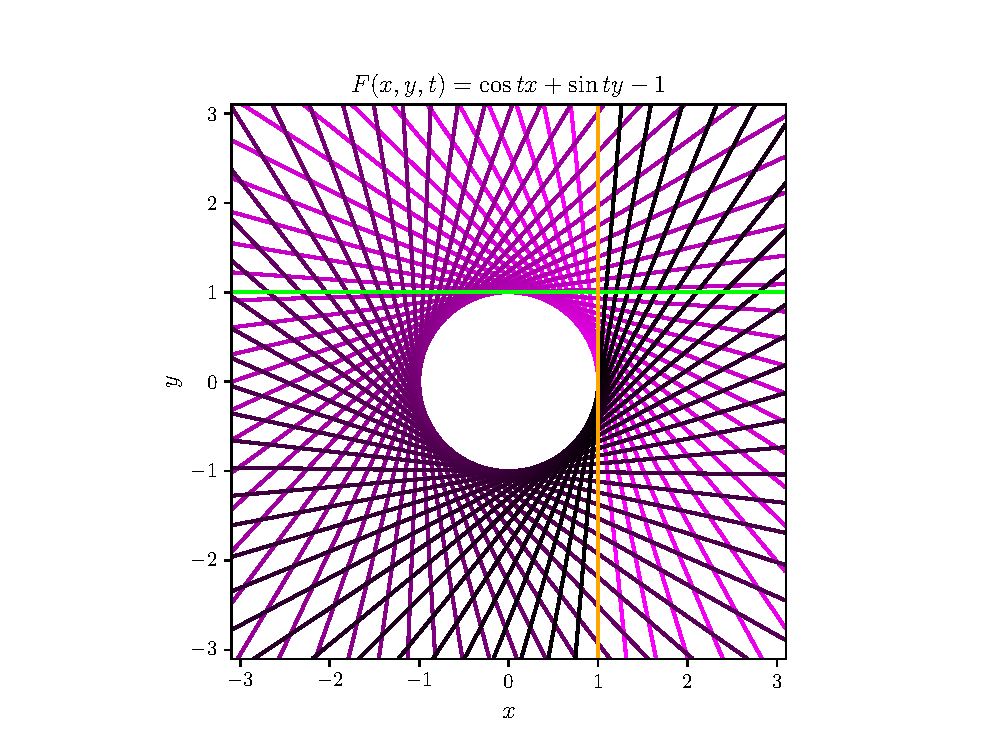
\includegraphics{images/lines_in_normal_form.eps}
	\caption[Systém priamok v normálovom tvare.]{Systém priamok v normálovom tvare zobrazený na intervale $[0, 2\pi]$ s krokom $\Delta t = 0,1$. Priamka $l$ je znázornená oranžovou farbou a transformovaná priamka $g_{\frac{\pi}{2}}(l)$ zelenou farbou.}
	\label{fig:lines_in_normal_form}
\end{figure}
\end{example}

Transformácie $g_{t}$ z príkladu sú prvkami špeciálna ortogonálnej grupy $SO(n)$. Táto grupa je Lieova grupa. Viac informácií o Lieovych grupách a Lieovych algebrách možno nájsť v \cite{Lee12}.
Použili sme štruktúru Lieovej grupy, aby sme opísali, ako sa grupa transformuje daný povrch. Ďalej, využijúc štruktúru hladkej variety môžeme opísať jednoparametrický systém plôch výlučne pomocou terminológie Lieových grúp. Táto teória sa aplikuje na nájdenie parametrizácie obálok kvadratických plôch v \cite{Vra22}. 

\subsection{Obálky a ODR}
Obálky súvisia aj so štúdiom obyčajných diferenciálnych rovníc, a najmä ich singulárnych riešení. Predpokladajme, že jednoparametrický systém kriviek $\mathcal{F}$ je riešením nejakej diferenciálnej rovnice prvého rádu. Potom môže existovať aj ďalšia krivka spĺňajúca túto diferenciálnu rovnicu, ktorá je dotyčnicou k $\mathcal{F}$ v každom bode. Táto krivka je obálka. V literatúre sa nazýva aj singulárne riešenie diferenciálnej rovnice.
Uvažujme ODR 
$$
\left(\frac{dy}{dx}\right)^2 - 4x\frac{dy}{dx} + 4y = 0.
$$
Jej regulárnym riešením sú integrálne krivky 
$$ y = - t^2 + 2tx, \text{ kde } t \in \mathbb{R}.$$
Riešenie môžeme reprezentovať ako jednoparametrický systém kriviek $\mathcal{F}$ s funkciou
$$F(x,y,t) = t^2 - 2tx + y. $$
Derivovaním podľa parametra $t$ dostávame
$$\dfrac{\partial F}{\partial t} (x,y,t) = 2t - 2x, $$
z čoho máme $t=x$ a dosadením do funkcie $F$ máme $F=-x^2+y,$ teda obálka je $y=x^2.$

Obálka tohto jednoparametrického systému priamok, ktorou je parabola $y = x^2$, rieši taktiež diferenciálnu rovnicu. Viac o tomto prístupe možno nájsť v \cite{Gro97}.

\begin{figure}[h]
	\centering
	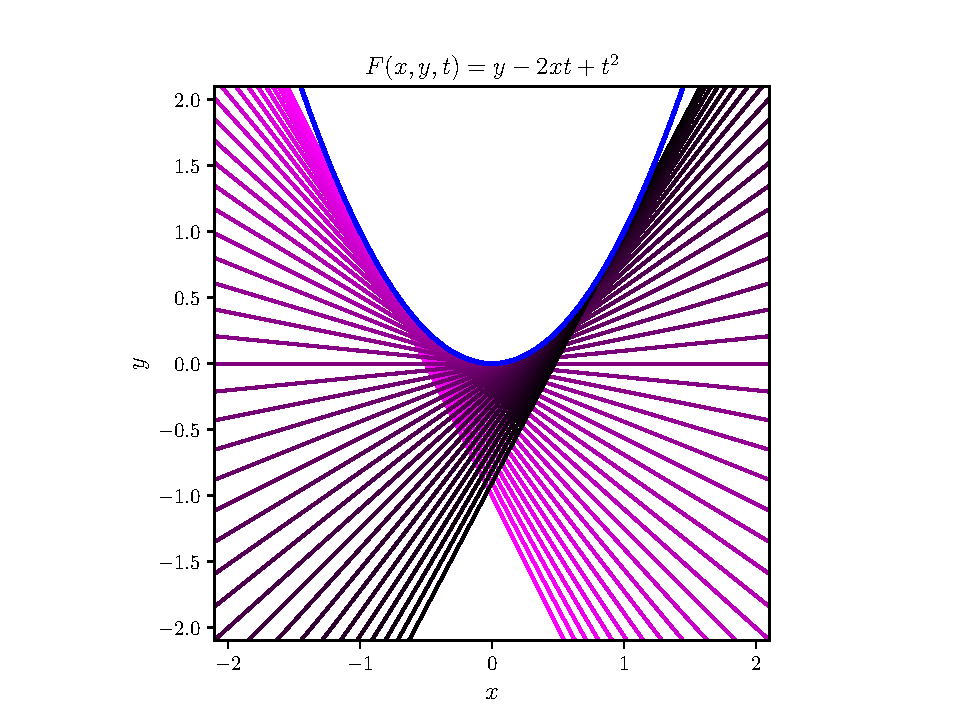
\includegraphics[trim={0 0.35cm 0 0.85cm},clip]{images/odr.pdf}
	\caption[Regulárne riešenia a obálka.]{Regulárne riešenia a obálka vykreslené na intervale $[-1,1]$ s krokom $\Delta t = 0,05$. Pre $t=-1$ je zobrazená časť priamky ružová, pre $t=1$ čierna, modrou farbou je vykreslená obálka.}
	\label{fig:odr}
\end{figure}

\subsection{Lokálne prieniky} \label{lokalne prieniky pre krivky}
Lokálny prienik systému kriviek $\mathcal{F} $ pozostáva z prienikov nekonečne blízkych susedných kriviek systému. Definujme túto myšlienku formálne.
\begin{definition}[Lokálny prienik] \label{def:lokalny prienik}
Lokálny prienik systému $\mathcal{F}$ je množina všetkých prienikov infinitezimálne blízkych prvkov pre všetky parametre $t \in I$. Označuje sa ako $\mathcal{L}$ a platí
$
\mathcal{L} := \bigcup_{t \in I} \mathcal{L}_{t}
$ kde
$$
\mathcal{L}_{t} = \lim_{\varepsilon \to 0} F_{t} \cap F_{t + \varepsilon}
$$
pre nejaké pevné $t \in I.$
\end{definition}
Lokálny priesečník regulárneho systému sa v mnohých prípadoch zhoduje s jeho obálkou. Ilustrujme to na nasledovnom príklade.

\begin{example}
Vezmime dva ľubovoľné, ale odlišné prvky systému $F(x, y, t) = y - 2tx - t.$
Pre fixné parametre $t_1 \neq t_2$ tak máme
$$F(x_1, y_1, t_1) = y_1 - 2t_1x_1 - t_1^2,$$
$$F(x_2, y_2, t_2) = y_2 - 2t_2x_2 - t_2^2.$$ 
Označme priesečník týchto dvoch priamok $Q = (q_x, q_y)^T.$ Pre priesečník $Q$ platí $$F(Q, t_1) = 0 = F(Q, t_2),$$ odkiaľ vyplýva 
$$(t_2 - t_1)(2q_x + t_1 + t_2) = 0.$$ 
Keďže podľa predpokladu $t_1 \neq t_2$, jediné riešenie tejto rovnice je $q_x = -\dfrac{t_1 + t_2}{2}$ a priesečník je potom daný 
$$Q = (-\dfrac{t_1 + t_2}{2}, -t_1t_2)^T.$$ Definujme $\varepsilon := t_2 - t_1$ a nechajme $\varepsilon$ smerovať k nule, dostávame priesečník
$$
\lim_{\varepsilon \to 0} 
\begin{pmatrix} 
-t_1 - \dfrac{\varepsilon}{2} \\
-t_1(t_1 + \varepsilon)
\end{pmatrix} = \begin{pmatrix} 
-t_1 \\
-t_1^2
\end{pmatrix}.
$$
Po reparametrizácii $t_1(t) = -t$ je ľahké vidieť, že množina všetkých týchto priesečníkov $\mathcal{L} = \{(t, -t^2): t \in \mathbb{R}\} = \mathcal{E}$, ktorá predstavuje lokálny priesečník, sa zhoduje s vypočítanou množinou bodov obálky.
\end{example}

\begin{corollary} Nech je daný systém $\mathcal{F}$. Každý bod lokálneho priesečníka systému $\mathcal{L}$ je aj bodom obálky systému $\mathcal{E}$. Teda platí
$$ \mathcal{L} \subseteq \mathcal{E}. $$
\end{corollary}

\begin{proof}
Pre každý bod $Q \in \mathcal{L}$ lokálneho prieniku systému $\mathcal{F}$ existuje podľa definície \ref{def:lokalny prienik} aspoň jedno $t_0 \in I,$ pre ktoré $Q \in \mathcal{L}_{t_0}, $ a teda $Q$ patrí do prieniku nekonečne blízkych prvkov pre $\mathcal{F}$ pre $t_0,$ to znamená, že platí
$$ F(Q, t_0) = \dfrac{\partial F}{\partial t} (Q, t_0) = 0,
$$  
čo je z definície \ref{charakterizacia} bod obálky $\mathcal{E}.$
\end{proof}

\section{Obálka sfér}
Označme $X \in \mathbb{R}^3$ a predpokladajme, že $m(t) \colon I \subset \mathbb{R} \rightarrow \mathbb{R}^3$ je parametrizácia krivky a $r(t) \colon I \rightarrow \mathbb{R}^{+}$ je funkcia definovaná na tom istom intervale. Krivka $m$ sa nazýva kostrová krivka obálky (\textit{spine curve}) a $r$ sa nazýva funkcia polomeru (\textit{radius function}). Jednoparametrický systém sfér $\mathcal{S}$ je daný rovnicou

$$
F(X, t) = \langle X - m(t), X - m(t) \rangle - r^2(t)= 0.
$$

Podľa definície \ref{charakterizacia}, obálku $\mathcal{E}$ možno nájsť ako prienik systému sfér $\mathcal{S}$ a ich derivácií $\mathcal{\dot{S}}$ pre všetky $t \in I$. Derivácia $\mathcal{S}$ nám dáva jednoparametrický systém rovín $\mathcal{\dot{S}}$ daný rovnicou

$$
\dfrac{\partial F}{\partial t} (X, t) = \langle \dot{m}(t), X - m(t) \rangle + r(t) \dot{r}(t) = 0.
$$
Pre nájdenie obálky $\mathcal{E}$ budeme teda hľadať prieniky sféry $\mathcal{S}_t$ a roviny $\mathcal{\dot{S}}_t $ pre každý parameter $t \in I$.

\section{Charakteristická kružnica}
\begin{definition}[Charakteristická kružnica]
V prípade, že pre $t \in I$ je $\mathcal{S}_{t} \cap \mathcal{\dot{S}}_{t} \neq \emptyset$, sa tento prienik nazýva sa charakteristická kružnica $c_{t}$. V prípade $\mathcal{S}_{t} \cap \mathcal{\dot{S}}_{t} = \emptyset$, pre \(t\) neexistuje žiadna charakteristická kružnica.
\end{definition}

\begin{lemma} \label{lema o zjednoteni charakteristickych kruznic}
Zjednotenie všetkých charakteristických kružníc $c_{t}$ jednoparametrického systému sfér $\mathcal{S}_t$ je obálka $\mathcal{E}$ tohto systému, teda platí $$\mathcal{E} = \bigcup_{t \in I} c_{t}.$$
\end{lemma}

\begin{proof}
Nech bod $X$ patrí do zjednotenia kružníc $ \bigcup_{t \in I} c_{t}, $ potom existuje aspoň jedno $t_0 \in I, $ pre ktoré $X \in c_{t_0}.$ Keďže $c_{t_0} = \mathcal{S}_{t_0} \cap \mathcal{\dot{S}}_{t_0}, $ tak sú rovnice $\mathcal{S}_{t_0} $ a $ \mathcal{\dot{S}}_{t_0}$ splnené pre nejaké $t_0$ a $X,$ a preto patrí $X$ obálke $\mathcal{E}, $ a teda platí inklúzia $\bigcup_{t \in I} c_{t} \subseteq \mathcal{E}. $

Opačne, ak $X$ patrí obálke $\mathcal{E},$ existuje podľa definície \ref{charakterizacia} $t_0 \in I $ také, že platí $F(X,t_0) = 0$ a súčasne $\dfrac{\partial F}{\partial t}(X, t_0)=0,$ to znamená, že $X$ leží v prieniku $\mathcal{S}_{t_0} \cap \mathcal{\dot{S}}_{t_0} = c_{t_0} $ a $c_{t_0} \subseteq \bigcup_{t \in I} c_t. $ Preto platí inklúzia $\mathcal{E} \subseteq \bigcup_{t \in I} c_t.$ 

Týmto je rovnosť $\mathcal{E} = \bigcup_{t \in I} c_t$ dokázaná.
\end{proof}

Obálka sfér sa teda skladá zo systému kružníc. Charakteristická kružnica leží celá v rovine $\mathcal{\dot{S}}_t $, takže v tejto rovine leží aj jej stred. Dotykový vektor kostrovej krivky $m(t)$ je kolmý na rovinu $\mathcal{\dot{S}}_t$, teda stred $C_t$ charakteristickej kružnice leží na dotyčnici $T(t, s)= m(t) + s \cdot \dot{m}(t),$ $s \in \mathbb{R}$, preto stred $C_t$ nájdeme ako
$$ \mathcal{\dot{S}}_t \cap T(t, s).$$
Pre parameter $s$ potom platí $s = \dfrac{r(t) \dot{r}(t)}{\langle \dot{m}(t), \dot{m}(t) \rangle }, $
po dosadení do $T(t, s)$ získavame
\begin{equation}
\label{eq:stred charakteristickej kruznice}
C_t = m(t) - \frac{r(t) \dot{r}(t)}{\langle \dot{m}(t), \dot{m}(t) \rangle} \dot{m}(t).
\end{equation}

Rozoberme si nasledujúce dva prípady
\begin{itemize}
\item Ak je funkcia polomeru $r(t)$ konštantná, $\dot{r} \equiv 0$ a rovina $\mathcal{\dot{S}}_t$ obsahuje stred sféry $M_t$ pre všetky $t \in I$, v tomto prípade možno obálku $\mathcal{E}$ považovať za posunutie (\textit{offset}) kostrovej krivky $m$. Tieto obálky sú známe ako rúrkové plochy (\textit{pipe surfaces}). Keďže rovina $\mathcal{\dot{S}}_t$ charakteristickej kružnice $c_t$ obsahuje stred sféry $M_t$ v každom $t \in I$, charakteristická krivka je hlavnou kružnicou sféry a obálka $\mathcal{E}$ je pokrytá jednoparametrickým systémom zhodných kružníc.
\item Ak funkcia polomeru $r(t)$ nie je konštantná, potom $\dot{r}(t) \neq 0$ a rovina $\mathcal{\dot{S}}_t$  neprechádza stredom sféry $M_t$. V tomto prípade obálka $\mathcal{E}$ patrí do triedy kanálových plôch.
\end{itemize}

Polomer $l_t$ charakteristiskej kružnice  možno vypočítať z pravouhlého trojuholníka $M_tC_tP,$ kde $P$ je ľubovoľný bod na charakteristickej kružnici $c_t$, a teda aj na sfére $\mathcal{S}_t.$
$$ l_t = \sqrt{r^2(t) - \|M_tC_t\|^2} = r(t) \sqrt{ 1 - \frac{\dot{r}^2(t)}{\langle \dot{m}(t), \dot{m}(t) \rangle}}. $$
V prípade, že $ \|M_tC_t\| > r(t)$, sféra $\mathcal{S}_t$ nemá s obálkou $\mathcal{E}$ reálny kontakt. 

\begin{example}
Uvažujme kostrovú krivku $m(t)$ a polomer $r(t)$
$$ 
m(t) = \begin{pmatrix} 0 \\ 0 \\ t \end{pmatrix} \quad \text{ a } \quad r(t) = \frac{t}{\sqrt{26}}.
$$
potom obálka systému je daná rovnicami
\begin{align*}
&\mathcal{S} \colon x^2 + y^2 + (z - t)^2 - \frac{t^2}{26} = 0, \\
&\mathcal{\dot{S}} \colon z - \frac{25}{26}t = 0. \\
\end{align*}
Počítajme $ \mathcal{S} \cap \mathcal{\dot{S}} $ pre všetky $t \in \mathbb{R}.$ Z druhej rovnice dostaneme $t = \frac{26}{25}z$. Po dosadení do prvej rovnice, dostávame implicitnú rovnicu pre obálku $\mathcal{E}$
$$
x^2 + y^2 - \frac{1}{25}z^2 = 0,
$$
čo je rovnica rotačného kužeľa.

Napríklad, pre $t = 1 \in I$ charakteristická krivka je prienikom dvoch plôch daných
\begin{align*}
&\mathcal{S}_1 \colon x^2 + y^2 + (z - 1)^2 - \frac{1}{26} = 0, \\
&\mathcal{\dot{S}}_1 \colon z - \frac{25}{26} = 0. \\
\end{align*}
Z toho môžeme usúdiť, že charakteristická krivka $c_1$ je kružnica so stredom v bode $C_1 = (0, 0, \frac{25}{26})$ v rovine $z = \frac{25}{26}$ a neprechádza stredom sféry $M_1 = m(1) = (0,0,1)$, polomer $c_1$ je $l_{1} = \frac{\sqrt{25}}{26}$. Vzdialenosť bodov $ \|M_tC_t\| = \frac{1}{26}$ a $r(1)= \frac{1}{\sqrt{26}}$, takže platí, že $r(1) > \|M_tC_t\|$ a sféra $\mathcal{S}_1$ má s obálkou $\mathcal{E}$ reálny kontakt.
\end{example}

Jedným z dôležitých výsledkov je, že kanálové plochy, definované ako obálka jednoparametrického systému sfér s racionálnou funkciou polomeru $r(t)$ a stredmi v racionálnej krivke $m(t)$ možno racionálne parametrizovať \cite{Pet97}.

Bohužiaľ, vo väčšine prípadov sú rovnice, ktoré charakterizujú obálky, príliš zložité a odvodiť z nich rovnicu obálky nie sme schopní.

Rúrkové povrchy sa často objavujú pri výrobe potrubia. Hladké spojenie medzi dvoma nie nevyhnutne valcovými rúrami $\mathcal{P}_1$ a $\mathcal{P}_2$ sa modeluje tak, aby bol prechod hladký, bez záhybov, vodotesný alebo dokonca aj parotesný. Na to sa používa technika \textit{rolling ball blends}, využívajúca nasledujúcu myšlienku: Kým sa sféra $S$ s konštantným alebo nekonštantným polomerom $r$ kotúľa na oboch rúrach súčasne, zanecháva stopu $s_i$ na oboch rúrach. Zmiešavacia plocha je tá časť obálky $\mathcal{E}$ jednoparametrického systému sfér, ktorá leží medzi dvoma stopami $s_1$ a $s_2$. Kostrová krivka obálky $\mathcal{E}$ je priesečníkom ekvidištánt \textit{(offsetov)} plôch $\mathcal{P}_1$ a $\mathcal{P}_2$ vo vzdialenosti $r$. Každá charakteristická krivka spája dva dotykové body zmiešavacej plochy a plochami $\mathcal{P}_1$ a $\mathcal{P}_2$, ktoré sa majú zmiešavať. Viac detailov možno nájsť v \cite{Kar00} a \cite{Ode20}. Na obrázku \ref{fig:rolling_ball_blends} vľavo je znázornená metóda so sférou s konštantným polomerom $r$, vpravo s nekonštantným.

\begin{figure}[h]
	\centering
	\includegraphics[width=\textwidth]{images/rolling_ball_blends.png}
	\caption[Technika rolling ball blends.]{Technika rolling ball blend s konštatným polomerom vľavo, s nekonštantným polomerom vpravo \cite{Rollingballblends}.}
	\label{fig:rolling_ball_blends}
\end{figure}